\documentclass[12pt,a4paper]{article}
\usepackage{geometry}
\usepackage{listings}
\usepackage[dvipdfmx]{graphicx}%
\usepackage{float}
\usepackage{textcomp}
\graphicspath{ {images/} }
\lstset{breaklines=true, frame=lrtb}
\geometry{left=1in, right=1in, top=1in, bottom=1in}
\begin{document}

\title{A Tool to Reduce Change Cost of Testing Resources}
\author{Ruide Li\\Yamamoto Lab.,\\Dept. of Information Engineering, \\School of Engineering, \\Nagoya University}
\date{}
\maketitle

\section{Abstract}

With the increasing development of information technology, no matter software or hardware, the upgrade and update are becoming more and more frequent. Also, as the functions of devices and software are incredibly numerous and complicated, in order to create reliable products, the cost of testing phase is approximately more than 50\% of total development cost of IT systems. Moreover, recent IT systems tend to depend on the execution environment. Therefore, testing of these systems are also depended on environment situations. This means that testing modern IT systems needs to concern on varieties of environmental resources for executing IT systems. Testing should be implemented by managing environmental resource variable changes, because the order of testing resources may affect the total testing cost. The testing resource preparation cost may change for each test cases according to the necessary environment for the execution. For different test cases need the change of resources, the testing cost will increase. So, it is necessary to make the test more efficient by minimizing the resource change cost. 

For instance, suppose there is a test for a software, which queries data from different tables from different databases. If we manage the objects in the same table to be tested together, we can save the cost of changing in and out of these databases and tables.

This paper presents a tool written in Python 3, which helps minimize the testing execution time of changing resources by extracting a minimum cost sequence for a set of test cases which depend on resources. There are two input for this tool: testing cases and relationship among resources (both in Excel sheet). And the output is the sequence of all testing cases of reduced cost. The purpose of this tool is to extract data matrix from Excel and minizing the change cost in testing phase.

This paper firstly gives the defination of test matrix and resource matrix and provides the way to extract these two kinds of matrix from the Excel sheet in this tool. Notice here that the resource matrix is a kind of compressed data from test matrix by identifying the test cases which has the same cost, hence we can simply test these cases together with no resource changing cost. Then, this paper discusses two algorithms (nearest neighbor algorithm and cheapest link algorithm) of the tool to minimize the cost, comparing the rationality and feasibility of these two approaches. And finally gives some further possilbility of improving this minimizing tool.

\section{Introduction}

This tool is trying to optimize the total time cost of testing phase, considering the effect of execution sequence. Therefore, we should focus on the resources of testing cases and change cost among resources. In this paper, we assume that the change cost of any resource is independent. As for the solution of dependent resources, it is usually posible to split the resource into independent elements. If we can put all the cost information into a matrix, this will become a question of minimizing the path in a matrix. This section gives some relating definations, which used in the development of this tool. 

\subsection{Data in Table}

\subsubsection{Testing Cases}

The data of testing cases is one of the input of this tool. That means, we get these data directly from developers or testers (usually in Excel). As we can know from the words, this kind of data is a list of all testing cases, commonly written in Excel in human language. Developers and testers test their systems by checking every single case in this list.   

Testing cases may include a large amount of information, sometimes more than the tool needs. So after getting the testing cases data, we need to manually delete some information (columns) we do not need, only remaning the "test case ID" and "resources", or the tool will not extracting data correctly.

Here shows an example of testing cases before and after deleting unnecessary columns (written in Japanese, provided by Veriserve Corporation). I simply deleted columns of C to K (in Figure 1), which present functions and purposes of each testing procedure.

\begin{figure}[H]
\centering
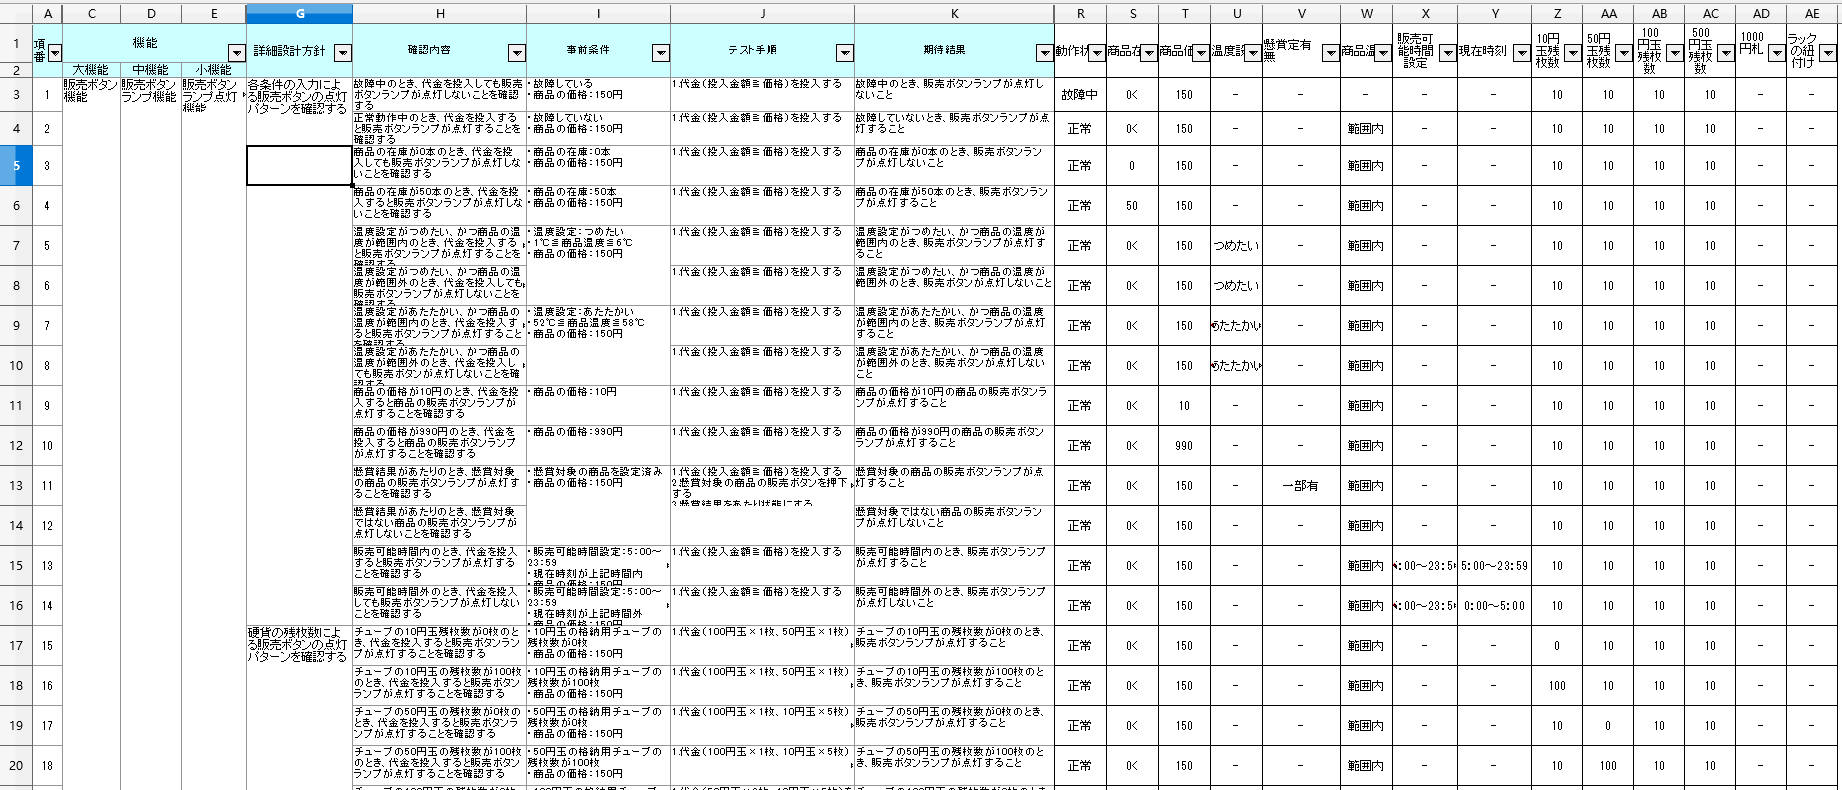
\includegraphics[width=0.9\textwidth]{testcases_bfdl.PNG}
\caption{Testing cases before deleting columns}
\end{figure}

\begin{figure}[H]
\centering
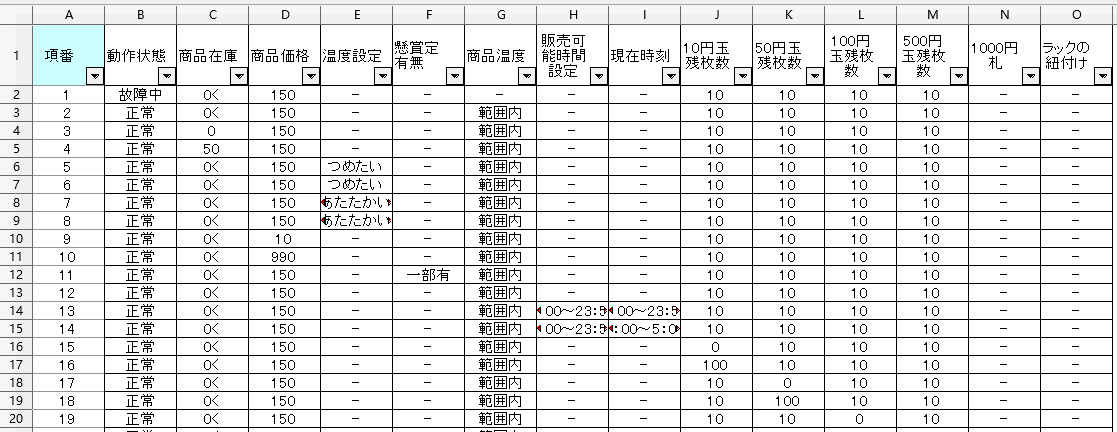
\includegraphics[width=0.9\textwidth]{testcases_afdl.PNG}
\caption{Testing cases after deleting columns}
\end{figure}

\subsubsection{Relationship among Resources}

The data of relationship among resources is the other input of this tool, also provided by developers or testers. During the development of this tool, relationship among resources is in another sheet in the same Excel file of testing cases. Notice that testing cases should be the first sheet, and relationship among resources should be the second sheet, since in the Excel-processing module of Python, sheets are identified in order, not by name.

In relationship among resources, it presents the cost of status change in each resource.

\begin{figure}[H]
\centering
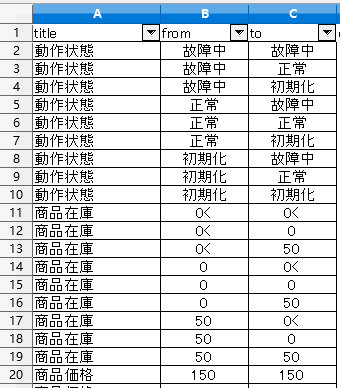
\includegraphics[width=0.4\textwidth]{resources_relation.PNG}
\caption{Relationship among Resources}
\end{figure}

In Figure 3 Line 18, for instance, we can know that the cost of changing "Stock" from "50" to "0" is "110". In this way, we can get every total cost from one testing case to another just by adding all cost of status change in each resource.

\subsubsection{Testing Resources}

Testing resources is a compressed data of testing cases, by identifying the same cost of testing cases. If two or more testing cases have the same cost at all resources, we put these testing cases into the same testing resource. As the cost of testing cases in the same testing resource is zero, we should make them tested together to optimize the total cost. However, testing resources is a little different from the data above, we have no need to make actual Excel data for it. It is just a kind of abstract concept helping us to understand the procedure.

\subsection{Data in Matrix}

\subsubsection{Test Matrix}

Since data in Excel is difficult to study and program, we need to intuitively extract the change cost into matrix form. Matrix files are saved in ".dat" file. Test matrix is a matrix extracted from testing cases and relationship among resources. It shows the change cost among all testing cases. For instance, the (\emph{i}, \emph{j}) element of the matrix represents the change cost from testing case \emph{i} to testing case \emph{j}. 

\subsubsection{Resource Matrix}

Resource matrix is a matrix extracted from testing resources. It shows the change cost among all testing resources. For instance, the (\emph{i}, \emph{j}) element of the matrix represents the change cost from testing resource \emph{i} to testing resource \emph{j}. 

\subsection{A Simple Example}

For understanding these definations above, here shows a simple example as following. Testing cases and relationship among resources are given as Table 1 and Table 2.

\begin{table}[htbp]
\parbox{.4\textwidth}{
\centering
\caption{Testing Cases}
\begin{tabular}{|l|l|l|}\hline
	ID & Table & Range\\\hline
	t0 & A & in\\\hline
	t1 & B & in\\\hline
	t2 & A & out\\\hline
	t3 & B & out\\\hline
	t4 & A & in\\\hline
	t5 & B & in\\\hline
	t6 & A & out\\\hline
	t7 & B & out\\\hline
\end{tabular}
}
\hfill
\parbox{.4\textwidth}{
\centering
\caption{Relationship among Resources}
\begin{tabular}{|l|l|l|l|}\hline
	Resource & From & To & Cost\\\hline
	Table & A & B & 2\\\hline
	Table & B & A & 3\\\hline
	Range & in & out & 1\\\hline
	Range & out & in & 2\\\hline
\end{tabular}
}
\end{table}

Then let us focus on the change cost from t7 to t0. In Table 1, we can find out that the resource change from t7 to t0 are table from B to A and range from out to in. So if we check Table 2, we can know that the total cost from t7 to t0 is 5. In this way, we can make the test matrix of Table 3.

Meanwhile, if we check testing cases more carefully, we can notice that t0 and t4 have the same resources. So we create a resource r0 for them, and create r1 = \{t1, t5\}, r2 = \{t2, t6\} and r3 = \{t3, t7\} for the rest of testing cases. And finally, we can make the resource matrix of Table 4 in the same way as test matrix. 

\begin{table}[htbp]
\parbox{.4\textwidth}{
\centering
\caption{Test Matrix}
\begin{tabular}{|c|cccccccc|}\hline
	 & t0 & t1 & t2 & t3 & t4 & t5 & t6 & t7 \\\hline
	t0 & 0 & 2 & 1 & 3 & 0 & 2 & 1 & 3\\
	t1 & 3 & 0 & 4 & 1 & 3 & 0 & 4 & 1\\
	t2 & 2 & 4 & 0 & 2 & 2 & 4 & 0 & 2\\
	t3 & 5 & 2 & 3 & 0 & 5 & 2 & 3 & 0\\
	t4 & 0 & 2 & 1 & 3 & 0 & 2 & 1 & 3\\
	t5 & 3 & 0 & 4 & 1 & 3 & 0 & 4 & 1\\
	t6 & 2 & 4 & 0 & 2 & 2 & 4 & 0 & 2\\
	t7 & 5 & 2 & 3 & 0 & 5 & 2 & 3 & 0\\\hline
\end{tabular}
}
\hfill
\parbox{.4\textwidth}{
\centering
\caption{Resources Matrix}
\begin{tabular}{|c|cccc|}\hline
	 & r0 & r1 & r2 & r3\\\hline
	r0 & 0 & 2 & 1 & 3\\
	r1 & 3 & 0 & 4 & 1\\
	r2 & 2 & 4 & 0 & 2\\
	r3 & 5 & 2 & 3 & 0\\\hline
\end{tabular}
}
\end{table}

From Table 3, we can find out that if we test in the given sequence (from t0 to t7), the cost is 2 + 4 + 2 + 5 + 2 + 4 +2 = 21. As for Table 4, we can know that if we test in the given sequence (from r0 to r3), the cost is 2 + 4 + 2 = 8, since changing cost of testing cases in the same testing resources is 0.

\section{Extracting Matrix from Excel}

As mentioned in the previous section, data of testing cases and relationship among resources are written in Excel, in order to make the data simplier to study and to be used by program, we need to extract matrix data from Excel. This section shows the approach to extract test matrix and resource matrix, and the result of extracting program. Notice that all programs in this paper are written in Python 3.4.3 enviornment and especially, Excel-processing programs (Appendix A and B) are using a Python module called "xlrd". Meanwhile, the programs are showing execution time, the computer used in the papper has the CPU of "Intel Core i7-6700 @ 3.40 GHz 3.40 GHz", 16.0GB RAM and OS of "Windows10 x64".

\subsection{Extracting Test Matrix}

Extracting test matrix is quite simple. The only thing we need to do is identifying all the resource status of each testing case and adding the cost together. In addition, in order to make comparison between the cost before and after using this tool, this program not only generates the matrix, but also computes the cost of all testing cases before optimizing.

Hence, for every (\emph{i}, \emph{j}) element in the matrix, the program checks every resource status in testing cases, queries the cost of status change in relation of resource, and add them together. The calculation of this algorithm is $$ TestingCases^2\times Resources\times Relations.$$

Execution result (Appendix A) on sample of Figure 2 and Figure 3 (Excel file "sample1.dat", 95 testing cases, 14 resources, 1459 relations) is as following.

\begin{lstlisting}
Time cost of extracting test matrix from Excel:
56.486727714538574  s

Test cost before minimizing:
10720
\end{lstlisting}

This means, if we do not optimize anything, just test in the sequence given, the cost is 10720.  Meanwhile, this program also generates a matrix data file ("matrix\_test1.dat").

\subsection{Extracting Resource Matrix}

To extract resource matrix, we should extract testing resources at first. The approach is searching all testing cases, if it belongs to a existing testing resource (having all the same resources), append the testing case into that testing resource, else create a new testng resource for it. And when generating resource matrix, it uses the same method as test matrix, just skipping the elements which are included in a testing resource. That is, for every (\emph{i}, \emph{j}) element in the matrix, the program checks every resource status in testing resources, queries the cost of status change in relation of resource, and add them together. The calculation of this algorithm is $$TestingResources^2\times Resources\times Relations.$$ 

Execution result (Appendix B) on sample of Figure 2 and Figure 3 (Excel file "sample1.dat", 95 testing cases, 14 resources, 1459 relations) is as following. The result shows all of the resources and their elements. For instance, testing cases 2, 12, 28, 29, 30, 31, 32, 34, 35, 36 are the elements of Resource 1.

\begin{lstlisting}
Resource 0 : [1]  Resource 1 : [2, 12, 28, 29, 30, 31, 32, 34, 35, 36]  Resource 2 : [3, 26]  Resource 3 : [4]  Resource 4 : [5, 6]  Resource 5 : [7, 8]  Resource 6 : [9]  Resource 7 : [10]  Resource 8 : [11]  Resource 9 : [13]  Resource 10 : [14]  Resource 11 : [15]  Resource 12 : [16]  Resource 13 : [17]  Resource 14 : [18]  Resource 15 : [19]  Resource 16 : [20]  Resource 17 : [21]  Resource 18 : [22]  Resource 19 : [23]  Resource 20 : [24]  Resource 21 : [25]  Resource 22 : [27, 33]  Resource 23 : [37, 38, 39, 41]  Resource 24 : [40, 42]  Resource 25 : [43]  Resource 26 : [44]  Resource 27 : [45]  Resource 28 : [46]  Resource 29 : [47]  Resource 30 : [48]  Resource 31 : [49]  Resource 32 : [50]  Resource 33 : [51]  Resource 34 : [52]  Resource 35 : [53]  Resource 36 : [54]  Resource 37 : [55]  Resource 38 : [56]  Resource 39 : [57]  Resource 40 : [58]  Resource 41 : [59]  Resource 42 : [60]  Resource 43 : [61]  Resource 44 : [62]  Resource 45 : [63]  Resource 46 : [64]  Resource 47 : [65]  Resource 48 : [66]  Resource 49 : [67]  Resource 50 : [68]  Resource 51 : [69]  Resource 52 : [70]  Resource 53 : [71]  Resource 54 : [72]  Resource 55 : [73]  Resource 56 : [74]  Resource 57 : [75]  Resource 58 : [76]  Resource 59 : [77]  Resource 60 : [78]  Resource 61 : [79]  Resource 62 : [80]  Resource 63 : [81]  Resource 64 : [82]  Resource 65 : [83]  Resource 66 : [84]  Resource 67 : [85]  Resource 68 : [86]  Resource 69 : [87]  Resource 70 : [88]  Resource 71 : [89]  Resource 72 : [90]  Resource 73 : [91]  Resource 74 : [92]  Resource 75 : [93]  Resource 76 : [94]  Resource 77 : [95]  
Time cost of extracting resource matrix from Excel:
37.508758306503296  s

Test cost after deleting cases in same resources:
9520
\end{lstlisting}

From this result, we can see that after compressing testing cases to testing resources, both the execution time and the total cost obviously decreased. Meanwhile, this program also generates a matrix data file ("matrix\_resource1.dat").

\section{Minimizing Algorithm}

After the matrices have been prepared, we need to use a certain algorithm to minimize the cost. In other words, we need to create a minized path (sequence) through the matrices. As is written in the previous section, we have 2 kind of matrices, the test matrix and the resource matrix. So we will input both of these 2 matrices into the minimizing tool, and see which matrix will lead to less cost. Here, we assume that resource matrix may lead to less cost, since the size of resource matrix is smaller and the given sequence is decreased.

When I firstly thought about the minimizing algorithm, I used repetitive nearest neighbor algorithm. However, during the test phase, I found that nearest neighbor algorithm does not always give the path at the least cost. This is reasonable, since nearest neighbor is just a sort of greedy algorithm. Therefore, I was wondering whether there is a method always outputing the least cost. As a result, after deeper study on the matrix, I have found that this problem is very close to, or we can call it an equivalence to travelling salesman problem (TSP, in addition, as the change cost is asymmetric, it belongs to the branch of aTSP). The only difference between this problem and TSP is that we have no need to go back to the point we start (but in some literatures, problems that not going back to the start are also included in TSP). Hence, we can see the testing cases/resources as vertexes (cities), and the cost between testing cases/resources as the weight of edges (distance between cities).

As is universally acknowledged, TSP is NP hard problem, having the complexity of $\mathcal{O}(n!)$, so using brute force algorithm to minimize the path is hopelessly inefficient. Therefore, although they cannot necessarily solve the problem, we have no choice but to use greedy algorithms.

In this section, we will discuss 2 kinds of greedy algorithms majorly used to solve TSP, repetitive nearest neighbor algorithm and cheapest link algorithm.

\subsection{Repetitive Nearest Neighbor Algorithm}

\subsubsection{Algorithm Description}

Nearest neighbor algorithm ($\mathcal{O}(n^2)$) is perhaps the simplest and most straightforward TSP approach. The key to this method is to always visit the nearest city. 

The algorithm shows as following:\cite{1}

\begin{enumerate}
\item Select a random city.
\item Find the nearest unvisited city and go there.
\item Are there any unvisitied cities left? If yes, repeat step 2.
\item Finish.
\end{enumerate}

But the simple nearest neighbor algorithm choose the start vertex randomly, so in order to make the result more close to optimal, it is better to choose repetitive nearest neighbor algorithm. The only difference is to loop all vertex as start. For exchange of the accuracy, the complexity becomes to $\mathcal{O}(n^3)$, but this is relatively acceptable.

The program min\_cost\_nn.py (Appendix C) extracts the sequence with minimized cost using repetitive nearest neighbor algorithm. 

\subsubsection{Execution of the Program}

Firstly, the program was tested on simple data.
The execution result of this program on the data in Table 3 is:

\begin{lstlisting}
min cost:  5
min path:  [0, 4, 6, 2, 7, 3, 5, 1]
\end{lstlisting}

The result shows that the optimized sequence is t0 \textrightarrow t4 \textrightarrow t6 \textrightarrow t2 \textrightarrow t7 \textrightarrow t3 \textrightarrow t5 \textrightarrow t1, and the total cost is 5. Comparing to the cost of 21 in given sequence in Section 2.3, this tool has reduced the testing cost by 76.19\%.

The execution result of this program on the data in Table 4 is:

\begin{lstlisting}
min cost:  5
min path:  [0, 2, 3, 1]
\end{lstlisting}

The result shows that the optimized sequence is r0 \textrightarrow r2 \textrightarrow r3 \textrightarrow r1, and the total cost is also 5. As we mentioned in Section 2.3, the resources are r0 = \{t0, t4\}, r1 = \{t1, t5\}, r2 = \{t2, t6\} and r3 = \{t3, t7\}. It is obvious that the result is actually the same as above. The cost also decrease by 76.19\%.

However, there is another problem in repetitive nearest neighbor algorithm. That is, if there are more than one equal minimum edge from a certain vertex, this algorithm cannot traversing all the vertex with minimum edge, but only choose the first minimum edge or the last one (depending on "\textless" or "\textless=" used in the "if" condition, Line 29, Appendix C). In our testing cases and testing resources data, equal change cost (although in different testing resources) happens a lot. So this situation will extremely affects the accuracy of the optimization. 

For instance, think about the matrix in Table 5. 

\begin{table}[htbp]
\centering
\caption{Nearest Neighbor Nonoptimal Matrix}
\begin{tabular}{|c|cccccc|}\hline
	 & t0 & t1 & t2 & t3 & t4 & t5 \\\hline
	t0 & 0 & 3 & 2 & 2 & 1 & 4\\
	t1 & 6 & 0 & 6 & 3 & 3 & 3\\
	t2 & 2 & 3 & 0 & 4 & 1 & 2\\
	t3 & 3 & 2 & 3 & 0 & 4 & 2\\
	t4 & 3 & 2 & 3 & 5 & 0 & 5\\
	t5 & 5 & 2 & 4 & 2 & 4 & 0\\\hline
\end{tabular}
\end{table}

The execution result of this program on the data in Table 5 is:

\begin{lstlisting}
min cost:  12
min path:  [0, 4, 1, 3, 5, 2]
\end{lstlisting}

However, think about the path of 0\textrightarrow4\textrightarrow1\textrightarrow5\textrightarrow3\textrightarrow2, the cost is 1 + 2 + 3 + 2 + 3 = 11. This is because the nearest neighbor algorithm do not make branches if it meet equal minimum edges, but only choose the first one or the last one it meets. So in order to consider all branches, I tried to make some improvement on this algorithm, and made a program of min\_cost\_nn\_v2.py (Appendix E) using recursive function. This program worked well when I tested it on simple data.

The execution result of this improved program on the data in Table 5 is:

\begin{lstlisting}
min cost path: [0, 4, 1, 5, 3, 2]
min cost: 11
\end{lstlisting}

Test on simple data only proves the rationality of the program, but do not guarantee any feasibility. Hence, test on large data should be necessary. Testing data used is the one showed in Figure 2 and 3, and we have already extracted matrices from it in Section 3. So we can just used those matrix data files as the input of the programs.

Although the improved program above (Appendix E) gives the result we expected, but unfortunately, when I tested it on large data, this program using recursive function cost unexpectedly massive amount of time to execute. Therefore, the only choice left is to accept that defect of nearest neighbor algorithm.

The execution result of min\_cost\_nn.py (Appendix C) on test matrix data ("matrix\_test1.dat") is: 

\begin{lstlisting}
min cost:  4893
min path:  [26, 41, 39, 32, 42, 94, 40, 93, 38, 92, 37, 91, 36, 90, 35, 89, 34, 88, 33, 87, 31, 86, 30, 85, 29, 84, 28, 83, 27, 82, 23, 81, 22, 80, 13, 79, 12, 78, 11, 77, 10, 76, 7, 75, 6, 74, 5, 73, 4, 72, 1, 71, 24, 0, 70, 14, 69, 25, 2, 68, 20, 67, 18, 66, 16, 65, 9, 64, 8, 63, 3, 62, 61, 15, 21, 60, 59, 58, 57, 47, 46, 55, 56, 53, 54, 19, 17, 45, 44, 43, 52, 51, 50, 49, 48]
execute time:  0.1787717342376709
\end{lstlisting}

The result shows the sequence of testing cases, and the total change cost is 4893. Comparing to the cost of 10720 in given sequence as mentioned in Section 3.1, this tool has decrease the testing cost by 54.36\%. 

The execution result of min\_cost\_nn.py (Appendix C) on resource matrix data ("matrix\_resource1.dat") is: 

\begin{lstlisting}
min cost:  6293
min path:  [22, 24, 25, 77, 23, 76, 20, 75, 19, 74, 10, 73, 9, 72, 8, 71, 5, 70, 4, 69, 1, 68, 21, 0, 67, 11, 66, 17, 65, 15, 64, 13, 63, 7, 62, 6, 61, 2, 60, 3, 59, 58, 57, 56, 55, 54, 53, 52, 51, 50, 49, 48, 47, 46, 45, 44, 12, 18, 43, 42, 41, 40, 30, 29, 38, 39, 36, 37, 16, 14, 28, 27, 26, 35, 34, 33, 32, 31]
execute time:  0.09236979484558105
\end{lstlisting}

The result shows the sequence of testing resources (detail of the resources is showed in Section 3.2), and the total change cost is 4893. Comparing to the cost of 10720 in given sequence as mentioned in Section 3.1, this tool has decrease the testing cost by 41.30\%. 

Comparing the execution on test matrix and resource matrix, we can find out that in repetitive nearest neighbor algorithm, although the execute time is compressed, our hypothesis of resource matrix leading to less cost is untenable. Thinking about the reason, since in actual large data, equal minimum edges from one vertex create extremely complex branches, if it does not search all minimun edge branches, the optimization will be affected by the sequence of data. This should be considered as a unignorable factor.

\subsection{Cheapest Link Algorithm}

\subsubsection{Algorithm Description}
As the nearest neighbor algorithm has the defect, I tried to find out any alternative algorithm. Cheapest link algorithm is another majorly used greedy algorithm to solve TSP. Cheapest link algorithm gradually constructs a path by repeatedly selecting the shortest edge and adding it to the path as long as it does not create a cycle with less than N (matrix size) edges, or increases the degree of any vertex to more than 2. We must not add the same edge twice of course. The complexity of cheapest link algorithm is $\mathcal{O}(n^2 \log_2 n)$

The algorithm shows as following:\cite{1}

\begin{enumerate}
\item Sort all edges.
\item Select the shortest edge and add it to our path if it does not
\begin{itemize}
	\item create a cycle with less than N (matrix size) edges
	\item increases the degree of any vertex to more than 2
\end{itemize} 
\item Are there any unvisitied vertexes left? If yes, repeat step 2.
\item Finish.
\end{enumerate}

After understanding the algorithm, it is clear that the edges in this algorithm are undirected, so this algorithm is only valid on symmetric TSP (weight of forward and backward are the same between two vertexes). Since the change cost of testing resources are varies between symmetric and asymmetric, this algorithm can only be used as an alternative on symmetric situation.

\subsubsection{Execution of the Program}

According the algorithm above, I made a program of min\_cost\_cl.py (Appendix D).

To test this program, I made a sample of symmetric matrix showing in Table 6.

\begin{table}[htbp]
\centering
\caption{Symmetric Matrix}
\begin{tabular}{|c|cccccc|}\hline
	 & t0 & t1 & t2 & t3 & t4 & t5 \\\hline
	t0 & 0 & 2 & 5 & 4 & 3 & 7\\
	t1 & 2 & 0 & 3 & 1 & 6 & 2\\
	t2 & 5 & 3 & 0 & 3 & 2 & 4\\
	t3 & 4 & 1 & 3 & 0 & 6 & 8\\
	t4 & 3 & 6 & 2 & 6 & 0 & 5\\
	t5 & 7 & 2 & 4 & 8 & 5 & 0\\\hline
\end{tabular}
\end{table}

The execution result of min\_cost\_cl.py (Appendix E) on symmetric matrix data ("symmetric.dat") is: 

\begin{lstlisting}
cost: 11
path:  [0, 4, 2, 3, 1, 5]
execute time:  0.0010077953338623047
\end{lstlisting}

To make comparison, the execution result of min\_cost\_nn.py (Appendix C) on symmetric matrix data ("symmetric.dat") is: 

\begin{lstlisting}
min cost:  11
min path:  [5, 1, 3, 2, 4, 0]
execute time:  0.0010461807250976562
\end{lstlisting}

The cost in given sequence on this symmetric matrix is 19. From the result, we can see that program using cheapest link algorithm actually reduces the change cost indeed. 

\section{Conclusion and Further Issues}

\subsection{Conclusion}

In general, there are two parts in this minimizing tool: the matrix extracting part and the minimizing part. First, we have successfully extracted test matrix and resource matrix from testing cases in Excel, saving the matrices in ".dat" files. And then, according to the two algorithm discussed, the minimizing program has been successfully developed. Furthermore, in order to fix the defect on searching all branches and obtain more optimal result, a improved version of repetitive nearest neighbor algorithm has also been made. However, as the program of cheapest link algorithm is only an alternative on symmetric data, and the improved version of nearest neighbor algorithm cost extremely massive amount of time on large scale data, repetitive nearest neighbor algorithm is obviously a more reasonable option. In spite of the defect, this tool is able to reduce the changing cost by 54.36\% on actual data.

In the beginning of Section 4, we assumed that if we extract resource matrix at first, execution on the resource matrix will always lead to better optimization, but in practice, the test has demonstrated that this hypothesis is untenable, although the change cost decreased by 11.19\% only by generating the resource matrix. Since in actual large data, equal minimum edges from one vertex create extremely complex branches, ignoring most branches may leads to a result that the optimization will affected by the given sequence of the data.

\subsection{Further Issues}

As for further possibility, there are two points as far as I can imagine.

First, saving the data of testing cases and relationship among resources into database instead of Excel file, as the standardized data may help to guarantee the accuracy of data extraction. Meanwhile, the execution time of data extraction may be reduced, because of the efficient index structure of database. In this way, extracting matrix from testing cases simply becomes to the assembly of SQL.

Second, applying path improvement algorithm for solving TSP. Because of the lack of optimization in path construction algorithms, there are several path improvement algorithms trying to make the solution more optimal. 

Path construction algorithms have one thing in commmon, they stop when a solution is found and never tries to improve it. The best path construction algorithms usually gets within 10-15\% of optimality. Therefore, once a path has been generated by some path construction algorithms, we might wish to improve that solution.

There are several ways to do this, but the most common ones are the 2-opt and 3-opt local searches. Their performances are somewhat linked to the construction algorithms used. Other ways of improving our solution is to do a tabu search using 2-opt and 3-opt moves. Simulated annealing also use these moves to find neighboring solutions. Genetic algorithms generally use the 2-opt move as a means of mutating the population.\cite{1}

If we apply any path improvement algorithm into this tool, we can obtain a test sequence much closer to optimal.

\section{Acknowledgement}
I would like to thank my supervisor, Prof. Shuichiro Yamamoto, for the patient guidance, encouragement and advice he has provided throughout my time as his student. I have been extremely lucky to have a supervisor who cared so much about my work, and who responded to my questions and queries so promptly.

And I must express my appreciation to Mr. Masahiro Fujita from Veriserve Corporation, for providing the sample data set of testing cases and relationship among resources, also for pointing out the defect of nearest neighbor algorithm.

\begin{thebibliography}{9}

\bibitem{1}
  Christian Nilsson, 
  \emph{Heuristics for the Traveling Salesman Problem}, 
  Linkoping University.

\end{thebibliography}

\lstset{numbers=left}
\renewcommand{\thesubsection}{\Alph{subsection}}
\section{Appendices}
\subsection{extract\_test.py}
\lstinputlisting[tabsize=2]{"extract_test.py"}
\subsection{extract\_resource.py}
\lstinputlisting[tabsize=2]{"extract_resource.py"}
\subsection{min\_cost\_nn.py}
\lstinputlisting[tabsize=2]{"min_cost_nn.py"}
\subsection{min\_cost\_cl.py}
\lstinputlisting[tabsize=2]{"min_cost_cl.py"}
\subsection{min\_cost\_nn\_v2.py}
\lstinputlisting[tabsize=2]{"min_cost_nn_v2.py"}

\end{document}